\documentclass{llncs}


\usepackage{hyperref}
\usepackage{graphicx}
\usepackage{multirow}
\usepackage[misc,geometry]{ifsym}

\usepackage{amsmath}
\usepackage{enumitem}
%\usepackage{amsfonts}
%\usepackage{amssymb}
%\usepackage{epstopdf}
%\usepackage{epsfig}

\begin{document}

\mainmatter 

\title{Parallel Global Optimization for Non-Convex Mixed-Integer Problems}
\author{Konstantin Barkalov \and Ilya Lebedev %\Letter 
\\
\email{konstantin.barkalov@itmm.unn.ru}}

\institute{
Lobachevsky State University of Nizhni Novgorod, Nizhni Novgorod, Russia
}

\maketitle

\begin{abstract}
In the present paper, the mixed-integer global optimization problems are considered. A novel 
deterministic algorithm for solving the problems of this class based on the information-statistical 
approach to solving the continuous global optimization problems has been proposed. The 
comparison of this algorithm with known analogs demonstrating the efficiency of the 
developed approach has been conducted. The stable operation of the algorithm was confirmed 
also by solving a series of several hundred mixed-integer global optimization problems. 

\keywords global optimization, non-convex constraints, mixed-integer problems.

\end{abstract}

\section{Introduction}\label{sec:intro}

In the present paper, the global optimization problems and the method of solving these ones are 
considered. The global optimization problems are the computation-costly ones since the global 
optimum is an integral characteristic of the problem being solved and requires the investigation 
of the whole search domain. 
%As a result, the search of the global optimum is reduced to the construction of a coverage (in general, a nonuniform one) of the space of parameters. 
The problems, in which some parameters can take the integer values only (mixed-integer global 
optimization problems) are of special interest because for these ones it is more difficult to build 
the estimates of the optimum as compared to the continuous problems.

A lot of publication have been devoted to the methods of solving the mixed-integer problems 
(see, for example, the reviews~\cite{Burer,Boukouvala}). The well known deterministic 
methods of solving the problems of this class are based, as a rule, on the Branch-and-Bound 
approach or on the Branch-and-Reduce one. Also, a number of the metaheuristic and genetic 
algorithms are known, which are based one way or another on the random search concept.
%  based ones, anyway, based on the ideas of random search.

In the present study, we proposed a novel deterministic method for solving the mixed-integer 
problems based on the information-statistical approach to solving the global optimization 
problems \cite{Strongin2000,Strongin2013}. The paper text reflecting the results of preliminary 
studies is composed as follows. First, an approach to solving the problems with continuous 
parameters has been considered, then its generalization for the mixed-integer problems was 
proposed. In the final section, the results of comparison of the proposed method with the 
known analogs are presented.

\section{Global optimization algorithm and dimension reduction}

Let us consider a multiextremal optimization problem in the form
\begin{gather}\label{problem}
\varphi(y^\ast)=\min{\left\{\varphi(y):y\in D, \; g_j(y)\leq 0, \; 1 \leq j \leq m\right\}},\\
D=\left\{y\in R^N: a_i\leq y_i \leq b_i, 1\leq i \leq N\right\}.\nonumber
\end{gather}
Suppose, that the objective function $\varphi(y)$ (henceforth denoted by $g_{m+1}(y)$) and
the left-hand sides $g_j(y), \; 1\leq j \leq m$, of the constraints satisfy the Lipschitz condition
\[ \left|g_j(y')-g_j(y'')\right| \leq L_j \left\|y'-y'' \right\|, \; y',y''\in D, \; 1\leq j \leq m+1, \]
with constants $L_j, \; 1 \leq j \leq m+1$, respectively,  
and may be multiextremal.

Using a continuous single-valued mapping $y(x)$  (Peano-type space-filling curve, or \textit{evolvent}) of the interval $[0,1]$ onto $D$, a multidimensional problem (\ref{problem}) can be reduced to a one-dimensional problem
\begin{equation}\label{problem1}
\varphi(y(x^\ast))= \min \left\{g_{m+1}(y(x)): x \in [0,1], \; g_i(y(x))\leq 0, \; 1 \leq i \leq m\right\}.
\end{equation}
The reduction of dimensionality matches the multidimensional problem with a Lipschitzian objective function and constraints with a one-dimensional problem where the respective functions satisfy the uniform H\"older condition (see \cite{Strongin2000}).

An efficient global search algorithm (GSA) for solving the constrained optimization problem 
(\ref{problem1}) has been developed at University of Nizhni Novgorod. 

%Описание индексного алгоритма

A detailed description 
of the algorithm and the corresponding convergence theory are presented in 
\cite{Strongin2000}.

\section{Global search algorithm for mixed-integer problems}

Now, let us consider a method of adaptation of GSA for solving the mixed-integer global 
optimization problems 
\begin{gather}\label{problem_i}
\min{\left\{ g_{m+1}(y):y\in D, \; g_j(y)\leq 0, \; 1 \leq j \leq m\right\}},\\
D=\left\{a_i\leq y_i \leq b_i, \; 1\leq i \leq N, \; y_j \in Z, \; j \in J, \; y_i \in R, \; i \notin J \right\}.\nonumber
\end{gather}

Let us formulate a set of problems based on the problem (\ref{problem_i})
\begin{gather}\label{problem_is}
\min{\left\{ g_{m+1}^s(y):y\in D, \; g_i^s(y)\leq 0, \; 1 \leq i \leq m\right\}},\\
D=\left\{ a_i\leq y_i \leq b_i, \;  y_i \in R, \; i \notin J \right\}, \; s\in\{1,...,S\}.\nonumber 
\end{gather}
Each of these problems corresponds to the initial problem (\ref{problem_i}) with some combination of 
integer parameters. The number of problems $S$ will correspond to the number of all possible 
combinations of the integer parameters.

Using the dimensionality reduction scheme utilizing the evolvent $y(x)$ 
%based on the set of problems (\ref{problem_is}),
one can compose a united problem 
\begin{equation}\label{problem_is1}
\min \left\{g_{m+1}^s(y^s(x)): x \in [0,S], \; g_i^s(y^s(x)) \leq 0, \; 1 \leq i \leq m\right\},
\end{equation}
where the mapping $y^s(x)$ is formed on the basis of initial evolvent $y(x)$ as follows
\[
y^s(x)=y(x-s), \; x\in[s-1,s],\; s\in\{1,...,S\}.
\]
The functions $g_i^s(y^s(x))$ can have the breaks at the points $s\in \{1,...,S-1\}$, therefore, 
these points were considered as the punctured ones, the values of the objective function and 
constraints at these points remain undefined.

As an illustration, Fig. \ref{fig:1} presents the plots of the functions corresponding to a 
problem with one continuous parameter and one binary parameter.

\begin{figure}[ht]
    \centering
    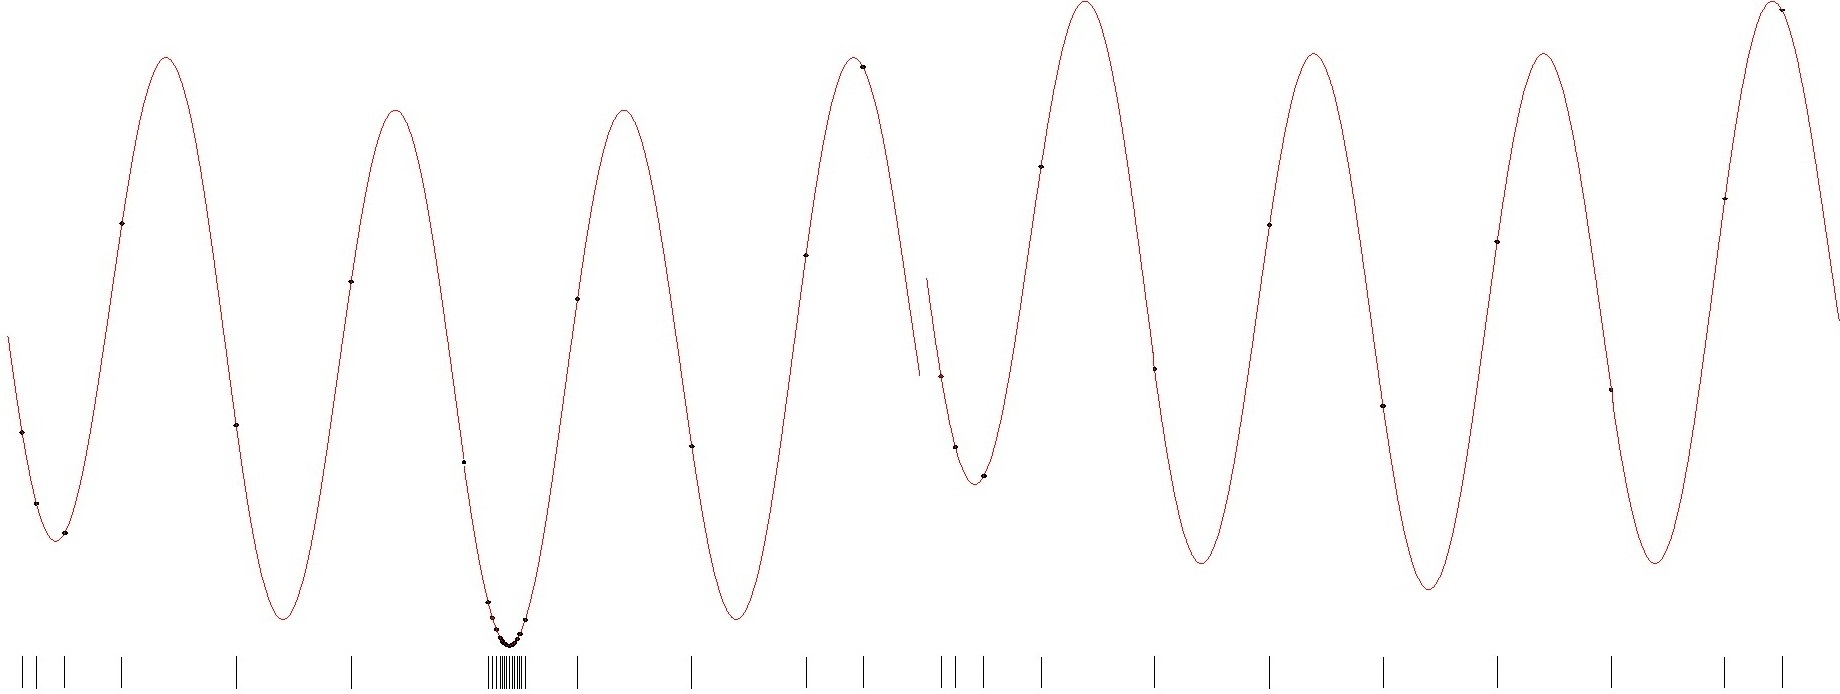
\includegraphics[height=2.9cm,width=0.8\textwidth]{fig1.jpg}
    \caption{Reduced mixed-integer global optimization problem}
    \label{fig:1}
\end{figure}

Applying the global search algorithm to solving the problem (\ref{problem_is1}), we will find 
the solution of the problem (\ref{problem_i}). In this case the major part of trials will conducted in 
the subproblem, the solving of which corresponds to the solving of the initial 
problem (\ref{problem_i}). In the rest subproblems, a only minor part of trials will be performed 
since the solutions of these subproblems are the locally optimal ones.
%with respect to the solution of the $s$-th subproblem. 
All the above is confirmed by Fig. \ref{fig:1}, where the  
points of trials executed in the course of solving this problem are denoted by the dashes.


Thus, we have constructed the \textit{Mixed-Integer Global Search Algorithm} (MIGSA) based on the  
reduction of the mixed-integer non-convex optimization problem to the non-convex optimization problem. 
%It is possible to prove that the convergence conditions for this algorithm will follow from the convergence conditions of its prototype (GSA).

\section{Results of experiments}

Let us compare the proposed MIGSA method with a genetic algorithm for solving the mixed-integer optimization problems implemented in Matlab Global Optimization Toolbox \cite{Matlab}. In Table 
\ref{tab:1}, the numbers of trials required for solving the known test mixed-integer 
problems by these methods are presented. For both methods, the same accuracy of search $10^{-2}$ were used. All numerical experiments were conducted on a 
computer with Intel Core i5-7300 2.5 GHz processor and 8 Gb RAM under MS Windows 10. The 
results of experiments have demonstrated the advantage to the MIGSA method in the number 
of iterations as well as in the execution time.

\begin{table}
	\caption{Comparison of MIGSA and GA}
	\label{tab:1}
	\center
	\begin{tabular}{cccccc}
		\hline\noalign{\smallskip}
	\multirow{2}{*}{Test problem}	 & \multicolumn{2}{c}{ GA } & & \multicolumn{2}{c}{MIGSA} \\
		\noalign{\smallskip} \cline{2-3} \cline{5-6} \noalign{\smallskip}
		 & $k$ & $t$ & & $k$ & $t$  \\
		\noalign{\smallskip} \hline \noalign{\smallskip}
		 Problem 2 \cite{Floudas}&	481 &	0.0601 & &	417 &	0.04 \\
%		 Problem 3 \cite{Floudas}& 	1821 &	0.1130 & & 3324 &	0.107 \\
		 Problem 6 \cite{Floudas}&	641 &	0.0510 & &	118 &	0.001 \\
		 Problem 1 \cite{Deep}   &	481 &	0.1378 & &	66 &	0.0007 \\
		 Problem 2 \cite{Deep}   &	481 &	0.0473 & &	57 &	0.0006 \\
		 Problem 7 \cite{Deep}   &	841 &	0.0736 & & 372	 &	0.017 \\
		\noalign{\smallskip}\hline
	\end{tabular}
\end{table}

In order to demonstrate the reliability of the MIGSA method, we have solved two series of 100 
multiextremal mixed-integer problems each constructed on the basis of modified problems of 
\textit{Simple} and \textit{Hard} classes generated by GKLS generator. %~\cite{Gaviano}. 
This generator of multiextremal functions is often used for the investigations of the global optimization algorithms~ 
\cite{Paulavicius2014,SergeyevKvasov2015,Lebedev2015,Gergel2015}.
In the problems generated in our experiments, there were 5 integer  and 3 continuous parameters.
The accuracy of the search %of the solution in the coordinates 
was equal to $10^{-2}$. All  
problems of the series have been solved successfully and for solving the problems based on 
the \textit{Simple} class 11988 trials in average were required whereas for solving the problems based 
on the \textit{Hard} class 24750 trials were required.


\textbf{Acknowledgments}. This study was supported by the Russian Science Foundation, project No 16-11-10150.

\begin{thebibliography}{10}

\bibitem{Burer}
Burer, S., Letchford, A.N.: Non-convex mixed-integer nonlinear programming: A survey. Surveys in Operations Research and Management Science \textbf{17}, 97--106 (2012) 

\bibitem{Boukouvala}
Boukouvala, F., Misener, R., Floudas, C.A.: Global optimization advances in Mixed-Integer Nonlinear Programming, MINLP, and Constrained Derivative-Free Optimization, CDFO. European J. Oper. Res. \textbf{252}, 701--727 (2016) 

\bibitem{Strongin2000}
Strongin, R.G., Sergeyev, Y.D.: Global optimization with non-convex constraints. Sequential and parallel algorithms. Kluwer Academic Publishers, Dordrecht (2000) %; DOI: 10.1007/978-1-4615-4677-1

\bibitem{Strongin2013}
Sergeyev, Ya.D., Strongin, R.G., Lera, D.: Introduction to global optimization exploiting space-filling curves. Springer (2013) %;  DOI: 10.1007/978-1-4614-8042-6

\bibitem{Floudas}
Floudas, C.A., Pardalos, P.M.:  Handbook of test problems in local and global optimization. Springer (1999)  %; DOI: 10.1007/978-1-4757-3040-1

\bibitem{Matlab}
https://www.mathworks.com/help/gads/mixed-integer-optimization.html

\bibitem{Deep}
Deep, K., Singh, K. P., Kansal, M.L., Mohan, C.: A real coded genetic algorithm for solving integer and mixed integer optimization problems. Appl. Math. Comput. \textbf{212}(2), 505--518 (2009)

%\bibitem{Gaviano} Gaviano, M., Kvasov, D.E, Lera, D., and Sergeyev, Ya.D.: Software for generation of classes of test functions with known local and global minima for global optimization. ACM Transactions on Mathematical Software \textbf{29}(4), 469--480 (2003)

\bibitem{Paulavicius2014} 
Paulavi\v{c}ius, R., Sergeyev, Y., Kvasov, D., \v{Z}ilinskas, J.: Globally-biased DISIMPL algorithm for expensive global optimization. J. Glob. Optim. \textbf{59}(2-3), 545--567 (2014)

\bibitem{SergeyevKvasov2015} 
Sergeyev, Y.D., Kvasov, D.E.: A deterministic global optimization using smooth diagonal auxiliary functions. Commun. Nonlinear. Sci. Numer. Simulat. \textbf{21}(1-3), 99--111 (2015)

\bibitem{Lebedev2015}
Lebedev, I., Gergel, V.: Heterogeneous parallel computations for solving global optimization problems. Procedia Computer Science \textbf{66}, 53--62 (2015)

\bibitem{Gergel2015}
Gergel, V., Sidorov, S.: A two-level parallel global search algorithm for solution of computationally intensive multiextremal optimization problems. Lecture Notes in Computer Science  \textbf{9251}, 505--515 (2015)


\end{thebibliography}


\end{document}
______________________________________________________________________
